\documentclass[1p]{elsarticle_modified}
%\bibliographystyle{elsarticle-num}

%\usepackage[colorlinks]{hyperref}
%\usepackage{abbrmath_seonhwa} %\Abb, \Ascr, \Acal ,\Abf, \Afrak
\usepackage{amsfonts}
\usepackage{amssymb}
\usepackage{amsmath}
\usepackage{amsthm}
\usepackage{scalefnt}
\usepackage{amsbsy}
\usepackage{kotex}
\usepackage{caption}
\usepackage{subfig}
\usepackage{color}
\usepackage{graphicx}
\usepackage{xcolor} %% white, black, red, green, blue, cyan, magenta, yellow
\usepackage{float}
\usepackage{setspace}
\usepackage{hyperref}

\usepackage{tikz}
\usetikzlibrary{arrows}

\usepackage{multirow}
\usepackage{array} % fixed length table
\usepackage{hhline}

%%%%%%%%%%%%%%%%%%%%%
\makeatletter
\renewcommand*\env@matrix[1][\arraystretch]{%
	\edef\arraystretch{#1}%
	\hskip -\arraycolsep
	\let\@ifnextchar\new@ifnextchar
	\array{*\c@MaxMatrixCols c}}
\makeatother %https://tex.stackexchange.com/questions/14071/how-can-i-increase-the-line-spacing-in-a-matrix
%%%%%%%%%%%%%%%

\usepackage[normalem]{ulem}

\newcommand{\msout}[1]{\ifmmode\text{\sout{\ensuremath{#1}}}\else\sout{#1}\fi}
%SOURCE: \msout is \stkout macro in https://tex.stackexchange.com/questions/20609/strikeout-in-math-mode

\newcommand{\cancel}[1]{
	\ifmmode
	{\color{red}\msout{#1}}
	\else
	{\color{red}\sout{#1}}
	\fi
}

\newcommand{\add}[1]{
	{\color{blue}\uwave{#1}}
}

\newcommand{\replace}[2]{
	\ifmmode
	{\color{red}\msout{#1}}{\color{blue}\uwave{#2}}
	\else
	{\color{red}\sout{#1}}{\color{blue}\uwave{#2}}
	\fi
}

\newcommand{\Sol}{\mathcal{S}} %segment
\newcommand{\D}{D} %diagram
\newcommand{\A}{\mathcal{A}} %arc


%%%%%%%%%%%%%%%%%%%%%%%%%%%%%5 test

\def\sl{\operatorname{\textup{SL}}(2,\Cbb)}
\def\psl{\operatorname{\textup{PSL}}(2,\Cbb)}
\def\quan{\mkern 1mu \triangleright \mkern 1mu}

\theoremstyle{definition}
\newtheorem{thm}{Theorem}[section]
\newtheorem{prop}[thm]{Proposition}
\newtheorem{lem}[thm]{Lemma}
\newtheorem{ques}[thm]{Question}
\newtheorem{cor}[thm]{Corollary}
\newtheorem{defn}[thm]{Definition}
\newtheorem{exam}[thm]{Example}
\newtheorem{rmk}[thm]{Remark}
\newtheorem{alg}[thm]{Algorithm}

\newcommand{\I}{\sqrt{-1}}
\begin{document}

%\begin{frontmatter}
%
%\title{Boundary parabolic representations of knots up to 8 crossings}
%
%%% Group authors per affiliation:
%\author{Yunhi Cho} 
%\address{Department of Mathematics, University of Seoul, Seoul, Korea}
%\ead{yhcho@uos.ac.kr}
%
%
%\author{Seonhwa Kim} %\fnref{s_kim}}
%\address{Center for Geometry and Physics, Institute for Basic Science, Pohang, 37673, Korea}
%\ead{ryeona17@ibs.re.kr}
%
%\author{Hyuk Kim}
%\address{Department of Mathematical Sciences, Seoul National University, Seoul 08826, Korea}
%\ead{hyukkim@snu.ac.kr}
%
%\author{Seokbeom Yoon}
%\address{Department of Mathematical Sciences, Seoul National University, Seoul, 08826,  Korea}
%\ead{sbyoon15@snu.ac.kr}
%
%\begin{abstract}
%We find all boundary parabolic representation of knots up to 8 crossings.
%
%\end{abstract}
%\begin{keyword}
%    \MSC[2010] 57M25 
%\end{keyword}
%
%\end{frontmatter}

%\linenumbers
%\tableofcontents
%
\newcommand\colored[1]{\textcolor{white}{\rule[-0.35ex]{0.8em}{1.4ex}}\kern-0.8em\color{red} #1}%
%\newcommand\colored[1]{\textcolor{white}{ #1}\kern-2.17ex	\textcolor{white}{ #1}\kern-1.81ex	\textcolor{white}{ #1}\kern-2.15ex\color{red}#1	}

{\Large $\underline{12a_{0078}~(K12a_{0078})}$}

\setlength{\tabcolsep}{10pt}
\renewcommand{\arraystretch}{1.6}
\vspace{1cm}\begin{tabular}{m{100pt}>{\centering\arraybackslash}m{274pt}}
\multirow{5}{120pt}{
	\centering
	\includegraphics[width=112pt]{../../../GIT/diagram.site/Diagrams/png/879_12a_0078.png}\\
\ \ \ A knot diagram\footnotemark}&
\allowdisplaybreaks
\textbf{Linearized knot diagam} \\
\cline{2-2}
 &
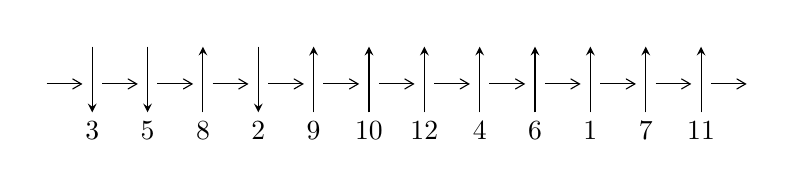
\begin{tikzpicture}[x=20pt, y=17pt]
	% nodes
	\node (C0) at (0, 0) {};
	\node (C1) at (1, 0) {};
	\node (C1U) at (1, +1) {};
	\node (C1D) at (1, -1) {3};

	\node (C2) at (2, 0) {};
	\node (C2U) at (2, +1) {};
	\node (C2D) at (2, -1) {5};

	\node (C3) at (3, 0) {};
	\node (C3U) at (3, +1) {};
	\node (C3D) at (3, -1) {8};

	\node (C4) at (4, 0) {};
	\node (C4U) at (4, +1) {};
	\node (C4D) at (4, -1) {2};

	\node (C5) at (5, 0) {};
	\node (C5U) at (5, +1) {};
	\node (C5D) at (5, -1) {9};

	\node (C6) at (6, 0) {};
	\node (C6U) at (6, +1) {};
	\node (C6D) at (6, -1) {10};

	\node (C7) at (7, 0) {};
	\node (C7U) at (7, +1) {};
	\node (C7D) at (7, -1) {12};

	\node (C8) at (8, 0) {};
	\node (C8U) at (8, +1) {};
	\node (C8D) at (8, -1) {4};

	\node (C9) at (9, 0) {};
	\node (C9U) at (9, +1) {};
	\node (C9D) at (9, -1) {6};

	\node (C10) at (10, 0) {};
	\node (C10U) at (10, +1) {};
	\node (C10D) at (10, -1) {1};

	\node (C11) at (11, 0) {};
	\node (C11U) at (11, +1) {};
	\node (C11D) at (11, -1) {7};

	\node (C12) at (12, 0) {};
	\node (C12U) at (12, +1) {};
	\node (C12D) at (12, -1) {11};
	\node (C13) at (13, 0) {};

	% arrows
	\draw[->,>={angle 60}]
	(C0) edge (C1) (C1) edge (C2) (C2) edge (C3) (C3) edge (C4) (C4) edge (C5) (C5) edge (C6) (C6) edge (C7) (C7) edge (C8) (C8) edge (C9) (C9) edge (C10) (C10) edge (C11) (C11) edge (C12) (C12) edge (C13) ;	\draw[->,>=stealth]
	(C1U) edge (C1D) (C2U) edge (C2D) (C3D) edge (C3U) (C4U) edge (C4D) (C5D) edge (C5U) (C6D) edge (C6U) (C7D) edge (C7U) (C8D) edge (C8U) (C9D) edge (C9U) (C10D) edge (C10U) (C11D) edge (C11U) (C12D) edge (C12U) ;
	\end{tikzpicture} \\
\hhline{~~} \\& 
\textbf{Solving Sequence} \\ \cline{2-2} 
 &
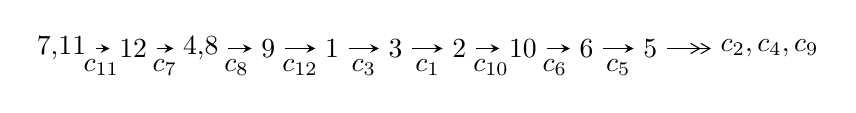
\begin{tikzpicture}[x=23pt, y=7pt]
	% node
	\node (A0) at (-1/8, 0) {7,11};
	\node (A1) at (1, 0) {12};
	\node (A2) at (33/16, 0) {4,8};
	\node (A3) at (25/8, 0) {9};
	\node (A4) at (33/8, 0) {1};
	\node (A5) at (41/8, 0) {3};
	\node (A6) at (49/8, 0) {2};
	\node (A7) at (57/8, 0) {10};
	\node (A8) at (65/8, 0) {6};
	\node (A9) at (73/8, 0) {5};
	\node (C1) at (1/2, -1) {$c_{11}$};
	\node (C2) at (3/2, -1) {$c_{7}$};
	\node (C3) at (21/8, -1) {$c_{8}$};
	\node (C4) at (29/8, -1) {$c_{12}$};
	\node (C5) at (37/8, -1) {$c_{3}$};
	\node (C6) at (45/8, -1) {$c_{1}$};
	\node (C7) at (53/8, -1) {$c_{10}$};
	\node (C8) at (61/8, -1) {$c_{6}$};
	\node (C9) at (69/8, -1) {$c_{5}$};
	\node (A10) at (11, 0) {$c_{2},c_{4},c_{9}$};

	% edge
	\draw[->,>=stealth]	
	(A0) edge (A1) (A1) edge (A2) (A2) edge (A3) (A3) edge (A4) (A4) edge (A5) (A5) edge (A6) (A6) edge (A7) (A7) edge (A8) (A8) edge (A9) ;
	\draw[->>,>={angle 60}]	
	(A9) edge (A10);
\end{tikzpicture} \\ 

\end{tabular} \\

\footnotetext{
The image of knot diagram is generated by the software ``\textbf{Draw programme}" developed by Andrew Bartholomew(\url{http://www.layer8.co.uk/maths/draw/index.htm\#Running-draw}), where we modified some parts for our purpose(\url{https://github.com/CATsTAILs/LinksPainter}).
}\phantom \\ \newline 
\centering \textbf{Ideals for irreducible components\footnotemark of $X_{\text{par}}$} 
 
\begin{align*}
I^u_{1}&=\langle 
- u^{81}- u^{80}+\cdots+b-1,\;u^{81}+u^{80}+\cdots+a+4 u,\;u^{82}+2 u^{81}+\cdots+u+1\rangle \\
I^u_{2}&=\langle 
- u^5+u^3- u^2+b- u,\;- u^7+u^5- u^4- u^3+a-1,\;u^8- u^7- u^6+2 u^5+u^4-2 u^3+2 u-1\rangle \\
\\
\end{align*}
\raggedright * 2 irreducible components of $\dim_{\mathbb{C}}=0$, with total 90 representations.\\
\footnotetext{All coefficients of polynomials are rational numbers. But the coefficients are sometimes approximated in decimal forms when there is not enough margin.}
\newpage
\renewcommand{\arraystretch}{1}
\centering \section*{I. $I^u_{1}= \langle - u^{81}- u^{80}+\cdots+b-1,\;u^{81}+u^{80}+\cdots+a+4 u,\;u^{82}+2 u^{81}+\cdots+u+1 \rangle$}
\flushleft \textbf{(i) Arc colorings}\\
\begin{tabular}{m{7pt} m{180pt} m{7pt} m{180pt} }
\flushright $a_{7}=$&$\begin{pmatrix}0\\u\end{pmatrix}$ \\
\flushright $a_{11}=$&$\begin{pmatrix}1\\0\end{pmatrix}$ \\
\flushright $a_{12}=$&$\begin{pmatrix}1\\- u^2\end{pmatrix}$ \\
\flushright $a_{4}=$&$\begin{pmatrix}- u^{81}- u^{80}+\cdots+5 u^2-4 u\\u^{81}+u^{80}+\cdots+u+1\end{pmatrix}$ \\
\flushright $a_{8}=$&$\begin{pmatrix}u\\- u^3+u\end{pmatrix}$ \\
\flushright $a_{9}=$&$\begin{pmatrix}- u^{14}+3 u^{12}-6 u^{10}+7 u^8-6 u^6+4 u^4-2 u^2+1\\- u^{14}+2 u^{12}-3 u^{10}+2 u^8+u^2\end{pmatrix}$ \\
\flushright $a_{1}=$&$\begin{pmatrix}- u^2+1\\- u^2\end{pmatrix}$ \\
\flushright $a_{3}=$&$\begin{pmatrix}- u^{81}-2 u^{80}+\cdots-4 u-1\\- u^{81}-2 u^{80}+\cdots+3 u^2-1\end{pmatrix}$ \\
\flushright $a_{2}=$&$\begin{pmatrix}u^{81}+u^{80}+\cdots+3 u+1\\- u^{76}+14 u^{74}+\cdots+4 u^3-4 u^2\end{pmatrix}$ \\
\flushright $a_{10}=$&$\begin{pmatrix}u^4- u^2+1\\u^4\end{pmatrix}$ \\
\flushright $a_{6}=$&$\begin{pmatrix}- u^9+2 u^7-3 u^5+2 u^3- u\\- u^9+u^7- u^5+u\end{pmatrix}$ \\
\flushright $a_{5}=$&$\begin{pmatrix}u^{19}-4 u^{17}+10 u^{15}-16 u^{13}+19 u^{11}-18 u^9+14 u^7-10 u^5+5 u^3-2 u\\u^{19}-3 u^{17}+6 u^{15}-7 u^{13}+5 u^{11}-3 u^9- u^3+u\end{pmatrix}$\\&\end{tabular}
\flushleft \textbf{(ii) Obstruction class $= -1$}\\~\\
\flushleft \textbf{(iii) Cusp Shapes $= 3 u^{81}+2 u^{80}+\cdots+19 u+9$}\\~\\
\newpage\renewcommand{\arraystretch}{1}
\flushleft \textbf{(iv) u-Polynomials at the component}\newline \\
\begin{tabular}{m{50pt}|m{274pt}}
Crossings & \hspace{64pt}u-Polynomials at each crossing \\
\hline $$\begin{aligned}c_{1}\end{aligned}$$&$\begin{aligned}
&u^{82}+35 u^{81}+\cdots+87 u+1
\end{aligned}$\\
\hline $$\begin{aligned}c_{2},c_{4}\end{aligned}$$&$\begin{aligned}
&u^{82}-9 u^{81}+\cdots-15 u+1
\end{aligned}$\\
\hline $$\begin{aligned}c_{3},c_{8}\end{aligned}$$&$\begin{aligned}
&u^{82}+u^{81}+\cdots-384 u+256
\end{aligned}$\\
\hline $$\begin{aligned}c_{5},c_{6},c_{9}\end{aligned}$$&$\begin{aligned}
&u^{82}-2 u^{81}+\cdots+231 u+49
\end{aligned}$\\
\hline $$\begin{aligned}c_{7},c_{11}\end{aligned}$$&$\begin{aligned}
&u^{82}+2 u^{81}+\cdots+u+1
\end{aligned}$\\
\hline $$\begin{aligned}c_{10},c_{12}\end{aligned}$$&$\begin{aligned}
&u^{82}-30 u^{81}+\cdots+u+1
\end{aligned}$\\
\hline
\end{tabular}\\~\\
\newpage\renewcommand{\arraystretch}{1}
\flushleft \textbf{(v) Riley Polynomials at the component}\newline \\
\begin{tabular}{m{50pt}|m{274pt}}
Crossings & \hspace{64pt}Riley Polynomials at each crossing \\
\hline $$\begin{aligned}c_{1}\end{aligned}$$&$\begin{aligned}
&y^{82}+33 y^{81}+\cdots-3371 y+1
\end{aligned}$\\
\hline $$\begin{aligned}c_{2},c_{4}\end{aligned}$$&$\begin{aligned}
&y^{82}-35 y^{81}+\cdots-87 y+1
\end{aligned}$\\
\hline $$\begin{aligned}c_{3},c_{8}\end{aligned}$$&$\begin{aligned}
&y^{82}-51 y^{81}+\cdots-1949696 y+65536
\end{aligned}$\\
\hline $$\begin{aligned}c_{5},c_{6},c_{9}\end{aligned}$$&$\begin{aligned}
&y^{82}-86 y^{81}+\cdots+637 y+2401
\end{aligned}$\\
\hline $$\begin{aligned}c_{7},c_{11}\end{aligned}$$&$\begin{aligned}
&y^{82}-30 y^{81}+\cdots+y+1
\end{aligned}$\\
\hline $$\begin{aligned}c_{10},c_{12}\end{aligned}$$&$\begin{aligned}
&y^{82}+46 y^{81}+\cdots+25 y+1
\end{aligned}$\\
\hline
\end{tabular}\\~\\
\newpage\flushleft \textbf{(vi) Complex Volumes and Cusp Shapes}
$$\begin{array}{c|c|c}  
\text{Solutions to }I^u_{1}& \I (\text{vol} + \sqrt{-1}CS) & \text{Cusp shape}\\
 \hline 
\begin{aligned}
u &= -0.742770 + 0.681590 I \\
a &= \phantom{-}0.244580 + 1.360110 I \\
b &= -0.293780 + 1.217510 I\end{aligned}
 & -3.63738 + 0.78744 I & \phantom{-0.000000 } 0 \\ \hline\begin{aligned}
u &= -0.742770 - 0.681590 I \\
a &= \phantom{-}0.244580 - 1.360110 I \\
b &= -0.293780 - 1.217510 I\end{aligned}
 & -3.63738 - 0.78744 I & \phantom{-0.000000 } 0 \\ \hline\begin{aligned}
u &= -0.983711 + 0.113504 I \\
a &= \phantom{-}1.135410 + 0.395982 I \\
b &= \phantom{-}1.160820 + 0.257051 I\end{aligned}
 & \phantom{-}5.61858 - 1.16403 I & \phantom{-0.000000 } 0 \\ \hline\begin{aligned}
u &= -0.983711 - 0.113504 I \\
a &= \phantom{-}1.135410 - 0.395982 I \\
b &= \phantom{-}1.160820 - 0.257051 I\end{aligned}
 & \phantom{-}5.61858 + 1.16403 I & \phantom{-0.000000 } 0 \\ \hline\begin{aligned}
u &= -0.972534 + 0.184730 I \\
a &= -1.180950 - 0.509477 I \\
b &= -1.235990 - 0.259714 I\end{aligned}
 & \phantom{-}4.40261 - 6.54773 I & \phantom{-0.000000 } 0 \\ \hline\begin{aligned}
u &= -0.972534 - 0.184730 I \\
a &= -1.180950 + 0.509477 I \\
b &= -1.235990 + 0.259714 I\end{aligned}
 & \phantom{-}4.40261 + 6.54773 I & \phantom{-0.000000 } 0 \\ \hline\begin{aligned}
u &= -0.555615 + 0.812609 I \\
a &= \phantom{-}0.41623 + 2.64855 I \\
b &= -2.05957 + 2.46409 I\end{aligned}
 & \phantom{-}6.23213 + 10.42700 I & \phantom{-0.000000 } 0 \\ \hline\begin{aligned}
u &= -0.555615 - 0.812609 I \\
a &= \phantom{-}0.41623 - 2.64855 I \\
b &= -2.05957 - 2.46409 I\end{aligned}
 & \phantom{-}6.23213 - 10.42700 I & \phantom{-0.000000 } 0 \\ \hline\begin{aligned}
u &= \phantom{-}0.673619 + 0.707958 I \\
a &= -0.84455 + 1.16088 I \\
b &= \phantom{-}0.674960 + 1.170380 I\end{aligned}
 & \phantom{-}0.191354 - 0.953328 I & \phantom{-0.000000 } 0 \\ \hline\begin{aligned}
u &= \phantom{-}0.673619 - 0.707958 I \\
a &= -0.84455 - 1.16088 I \\
b &= \phantom{-}0.674960 - 1.170380 I\end{aligned}
 & \phantom{-}0.191354 + 0.953328 I & \phantom{-0.000000 } 0\\
 \hline 
 \end{array}$$\newpage$$\begin{array}{c|c|c}  
\text{Solutions to }I^u_{1}& \I (\text{vol} + \sqrt{-1}CS) & \text{Cusp shape}\\
 \hline 
\begin{aligned}
u &= \phantom{-}0.779687 + 0.667468 I \\
a &= \phantom{-}0.42764 - 2.37824 I \\
b &= -2.31222 - 1.69191 I\end{aligned}
 & -4.10775 + 1.34673 I & \phantom{-0.000000 } 0 \\ \hline\begin{aligned}
u &= \phantom{-}0.779687 - 0.667468 I \\
a &= \phantom{-}0.42764 + 2.37824 I \\
b &= -2.31222 + 1.69191 I\end{aligned}
 & -4.10775 - 1.34673 I & \phantom{-0.000000 } 0 \\ \hline\begin{aligned}
u &= -0.540301 + 0.807682 I \\
a &= -0.36241 - 2.48744 I \\
b &= \phantom{-}2.13262 - 2.27043 I\end{aligned}
 & \phantom{-}8.19364 + 4.30348 I & \phantom{-0.000000 } 0 \\ \hline\begin{aligned}
u &= -0.540301 - 0.807682 I \\
a &= -0.36241 + 2.48744 I \\
b &= \phantom{-}2.13262 + 2.27043 I\end{aligned}
 & \phantom{-}8.19364 - 4.30348 I & \phantom{-0.000000 } 0 \\ \hline\begin{aligned}
u &= -0.825888 + 0.624112 I \\
a &= -0.354205 - 0.713190 I \\
b &= -0.024309 - 0.522887 I\end{aligned}
 & -1.70128 - 2.34818 I & \phantom{-0.000000 } 0 \\ \hline\begin{aligned}
u &= -0.825888 - 0.624112 I \\
a &= -0.354205 + 0.713190 I \\
b &= -0.024309 + 0.522887 I\end{aligned}
 & -1.70128 + 2.34818 I & \phantom{-0.000000 } 0 \\ \hline\begin{aligned}
u &= \phantom{-}0.722897 + 0.746924 I \\
a &= \phantom{-}1.37403 - 1.51592 I \\
b &= -0.61425 - 1.93274 I\end{aligned}
 & -1.47202 - 5.71308 I & \phantom{-0.000000 } 0 \\ \hline\begin{aligned}
u &= \phantom{-}0.722897 - 0.746924 I \\
a &= \phantom{-}1.37403 + 1.51592 I \\
b &= -0.61425 + 1.93274 I\end{aligned}
 & -1.47202 + 5.71308 I & \phantom{-0.000000 } 0 \\ \hline\begin{aligned}
u &= \phantom{-}0.540413 + 0.787249 I \\
a &= -0.992598 - 0.687172 I \\
b &= -0.759757 + 0.395132 I\end{aligned}
 & \phantom{-}2.76485 - 3.98227 I & \phantom{-0.000000 } 0 \\ \hline\begin{aligned}
u &= \phantom{-}0.540413 - 0.787249 I \\
a &= -0.992598 + 0.687172 I \\
b &= -0.759757 - 0.395132 I\end{aligned}
 & \phantom{-}2.76485 + 3.98227 I & \phantom{-0.000000 } 0\\
 \hline 
 \end{array}$$\newpage$$\begin{array}{c|c|c}  
\text{Solutions to }I^u_{1}& \I (\text{vol} + \sqrt{-1}CS) & \text{Cusp shape}\\
 \hline 
\begin{aligned}
u &= \phantom{-}0.936730 + 0.474455 I \\
a &= \phantom{-}0.714457 + 0.315117 I \\
b &= \phantom{-}1.46416 - 1.29373 I\end{aligned}
 & \phantom{-}2.91414 - 0.93006 I & \phantom{-0.000000 } 0 \\ \hline\begin{aligned}
u &= \phantom{-}0.936730 - 0.474455 I \\
a &= \phantom{-}0.714457 - 0.315117 I \\
b &= \phantom{-}1.46416 + 1.29373 I\end{aligned}
 & \phantom{-}2.91414 + 0.93006 I & \phantom{-0.000000 } 0 \\ \hline\begin{aligned}
u &= \phantom{-}0.608329 + 0.721946 I \\
a &= -0.607735 + 0.576661 I \\
b &= \phantom{-}0.243718 + 0.648491 I\end{aligned}
 & \phantom{-}0.322998 - 0.904010 I & \phantom{-}10.47601 + 0. I\phantom{ +0.000000I} \\ \hline\begin{aligned}
u &= \phantom{-}0.608329 - 0.721946 I \\
a &= -0.607735 - 0.576661 I \\
b &= \phantom{-}0.243718 - 0.648491 I\end{aligned}
 & \phantom{-}0.322998 + 0.904010 I & \phantom{-}10.47601 + 0. I\phantom{ +0.000000I} \\ \hline\begin{aligned}
u &= -0.532481 + 0.772000 I \\
a &= -0.21660 + 2.33589 I \\
b &= -2.78716 + 1.94540 I\end{aligned}
 & \phantom{-}1.25959 + 1.45124 I & \phantom{-}7.57778 + 0. I\phantom{ +0.000000I} \\ \hline\begin{aligned}
u &= -0.532481 - 0.772000 I \\
a &= -0.21660 - 2.33589 I \\
b &= -2.78716 - 1.94540 I\end{aligned}
 & \phantom{-}1.25959 - 1.45124 I & \phantom{-}7.57778 + 0. I\phantom{ +0.000000I} \\ \hline\begin{aligned}
u &= -0.489775 + 0.784882 I \\
a &= -0.27408 - 1.70120 I \\
b &= \phantom{-}2.05575 - 1.44650 I\end{aligned}
 & \phantom{-}8.50290 - 1.07286 I & \phantom{-}10.21024 + 0. I\phantom{ +0.000000I} \\ \hline\begin{aligned}
u &= -0.489775 - 0.784882 I \\
a &= -0.27408 + 1.70120 I \\
b &= \phantom{-}2.05575 + 1.44650 I\end{aligned}
 & \phantom{-}8.50290 + 1.07286 I & \phantom{-}10.21024 + 0. I\phantom{ +0.000000I} \\ \hline\begin{aligned}
u &= \phantom{-}0.512685 + 0.769270 I \\
a &= \phantom{-}0.731052 + 0.931298 I \\
b &= \phantom{-}0.784174 - 0.176818 I\end{aligned}
 & \phantom{-}2.94847 + 0.98484 I & \phantom{-}6.99928 - 2.55231 I \\ \hline\begin{aligned}
u &= \phantom{-}0.512685 - 0.769270 I \\
a &= \phantom{-}0.731052 - 0.931298 I \\
b &= \phantom{-}0.784174 + 0.176818 I\end{aligned}
 & \phantom{-}2.94847 - 0.98484 I & \phantom{-}6.99928 + 2.55231 I\\
 \hline 
 \end{array}$$\newpage$$\begin{array}{c|c|c}  
\text{Solutions to }I^u_{1}& \I (\text{vol} + \sqrt{-1}CS) & \text{Cusp shape}\\
 \hline 
\begin{aligned}
u &= -1.08016\phantom{ +0.000000I} \\
a &= \phantom{-}0.460931\phantom{ +0.000000I} \\
b &= \phantom{-}0.497360\phantom{ +0.000000I}\end{aligned}
 & \phantom{-}5.68315\phantom{ +0.000000I} & \phantom{-0.000000 } 0 \\ \hline\begin{aligned}
u &= -0.891351 + 0.616034 I \\
a &= -0.632357 - 0.558408 I \\
b &= -0.062681 - 0.410371 I\end{aligned}
 & -1.49964 - 2.51086 I & \phantom{-0.000000 } 0 \\ \hline\begin{aligned}
u &= -0.891351 - 0.616034 I \\
a &= -0.632357 + 0.558408 I \\
b &= -0.062681 + 0.410371 I\end{aligned}
 & -1.49964 + 2.51086 I & \phantom{-0.000000 } 0 \\ \hline\begin{aligned}
u &= -0.469791 + 0.773485 I \\
a &= \phantom{-}0.305390 + 1.361410 I \\
b &= -1.91125 + 1.15480 I\end{aligned}
 & \phantom{-}6.75343 - 7.22433 I & \phantom{-}8.05200 + 5.28342 I \\ \hline\begin{aligned}
u &= -0.469791 - 0.773485 I \\
a &= \phantom{-}0.305390 - 1.361410 I \\
b &= -1.91125 - 1.15480 I\end{aligned}
 & \phantom{-}6.75343 + 7.22433 I & \phantom{-}8.05200 - 5.28342 I \\ \hline\begin{aligned}
u &= \phantom{-}0.963981 + 0.534698 I \\
a &= -1.006010 - 0.207935 I \\
b &= -1.58881 + 1.45848 I\end{aligned}
 & \phantom{-}3.33664 + 4.49587 I & \phantom{-0.000000 } 0 \\ \hline\begin{aligned}
u &= \phantom{-}0.963981 - 0.534698 I \\
a &= -1.006010 + 0.207935 I \\
b &= -1.58881 - 1.45848 I\end{aligned}
 & \phantom{-}3.33664 - 4.49587 I & \phantom{-0.000000 } 0 \\ \hline\begin{aligned}
u &= -0.831377 + 0.727164 I \\
a &= -0.694470 + 1.035420 I \\
b &= -0.983570 + 0.376220 I\end{aligned}
 & -3.10733 - 4.66813 I & \phantom{-0.000000 } 0 \\ \hline\begin{aligned}
u &= -0.831377 - 0.727164 I \\
a &= -0.694470 - 1.035420 I \\
b &= -0.983570 - 0.376220 I\end{aligned}
 & -3.10733 + 4.66813 I & \phantom{-0.000000 } 0 \\ \hline\begin{aligned}
u &= \phantom{-}0.869045 + 0.089866 I \\
a &= -0.106416 + 0.510526 I \\
b &= \phantom{-}0.181534 - 0.847373 I\end{aligned}
 & \phantom{-}1.05325 + 1.74872 I & \phantom{-}11.28230 - 4.54859 I\\
 \hline 
 \end{array}$$\newpage$$\begin{array}{c|c|c}  
\text{Solutions to }I^u_{1}& \I (\text{vol} + \sqrt{-1}CS) & \text{Cusp shape}\\
 \hline 
\begin{aligned}
u &= \phantom{-}0.869045 - 0.089866 I \\
a &= -0.106416 - 0.510526 I \\
b &= \phantom{-}0.181534 + 0.847373 I\end{aligned}
 & \phantom{-}1.05325 - 1.74872 I & \phantom{-}11.28230 + 4.54859 I \\ \hline\begin{aligned}
u &= \phantom{-}0.914722 + 0.658273 I \\
a &= \phantom{-}2.36183 - 0.57009 I \\
b &= \phantom{-}1.43535 - 3.27787 I\end{aligned}
 & -3.69309 + 3.79631 I & \phantom{-0.000000 } 0 \\ \hline\begin{aligned}
u &= \phantom{-}0.914722 - 0.658273 I \\
a &= \phantom{-}2.36183 + 0.57009 I \\
b &= \phantom{-}1.43535 + 3.27787 I\end{aligned}
 & -3.69309 - 3.79631 I & \phantom{-0.000000 } 0 \\ \hline\begin{aligned}
u &= \phantom{-}1.13174\phantom{ +0.000000I} \\
a &= -2.77777\phantom{ +0.000000I} \\
b &= -0.171583\phantom{ +0.000000I}\end{aligned}
 & \phantom{-}6.95973\phantom{ +0.000000I} & \phantom{-0.000000 } 0 \\ \hline\begin{aligned}
u &= -0.879897 + 0.717160 I \\
a &= \phantom{-}1.072790 - 0.475215 I \\
b &= \phantom{-}0.915535 + 0.286937 I\end{aligned}
 & -2.95968 - 0.83056 I & \phantom{-0.000000 } 0 \\ \hline\begin{aligned}
u &= -0.879897 - 0.717160 I \\
a &= \phantom{-}1.072790 + 0.475215 I \\
b &= \phantom{-}0.915535 - 0.286937 I\end{aligned}
 & -2.95968 + 0.83056 I & \phantom{-0.000000 } 0 \\ \hline\begin{aligned}
u &= -1.136470 + 0.010119 I \\
a &= \phantom{-}0.107222 + 0.732042 I \\
b &= \phantom{-}0.127712 + 0.826867 I\end{aligned}
 & \phantom{-}8.58956 - 2.55565 I & \phantom{-0.000000 } 0 \\ \hline\begin{aligned}
u &= -1.136470 - 0.010119 I \\
a &= \phantom{-}0.107222 - 0.732042 I \\
b &= \phantom{-}0.127712 - 0.826867 I\end{aligned}
 & \phantom{-}8.58956 + 2.55565 I & \phantom{-0.000000 } 0 \\ \hline\begin{aligned}
u &= \phantom{-}1.146400 + 0.030933 I \\
a &= -2.25094 + 0.29979 I \\
b &= -0.481995 - 0.450536 I\end{aligned}
 & \phantom{-}12.2980 + 9.0487 I & \phantom{-0.000000 } 0 \\ \hline\begin{aligned}
u &= \phantom{-}1.146400 - 0.030933 I \\
a &= -2.25094 - 0.29979 I \\
b &= -0.481995 + 0.450536 I\end{aligned}
 & \phantom{-}12.2980 - 9.0487 I & \phantom{-0.000000 } 0\\
 \hline 
 \end{array}$$\newpage$$\begin{array}{c|c|c}  
\text{Solutions to }I^u_{1}& \I (\text{vol} + \sqrt{-1}CS) & \text{Cusp shape}\\
 \hline 
\begin{aligned}
u &= \phantom{-}1.149210 + 0.018459 I \\
a &= \phantom{-}2.36564 - 0.19446 I \\
b &= \phantom{-}0.488971 + 0.274865 I\end{aligned}
 & \phantom{-}14.1727 + 2.8208 I & \phantom{-0.000000 } 0 \\ \hline\begin{aligned}
u &= \phantom{-}1.149210 - 0.018459 I \\
a &= \phantom{-}2.36564 + 0.19446 I \\
b &= \phantom{-}0.488971 - 0.274865 I\end{aligned}
 & \phantom{-}14.1727 - 2.8208 I & \phantom{-0.000000 } 0 \\ \hline\begin{aligned}
u &= -0.938888 + 0.666226 I \\
a &= \phantom{-}1.169250 + 0.543123 I \\
b &= \phantom{-}0.099267 + 0.943058 I\end{aligned}
 & -3.04447 - 6.00273 I & \phantom{-0.000000 } 0 \\ \hline\begin{aligned}
u &= -0.938888 - 0.666226 I \\
a &= \phantom{-}1.169250 - 0.543123 I \\
b &= \phantom{-}0.099267 - 0.943058 I\end{aligned}
 & -3.04447 + 6.00273 I & \phantom{-0.000000 } 0 \\ \hline\begin{aligned}
u &= \phantom{-}0.974939 + 0.669400 I \\
a &= -1.18700 + 0.86217 I \\
b &= -0.31958 + 2.22104 I\end{aligned}
 & \phantom{-}1.07667 + 6.24979 I & \phantom{-0.000000 } 0 \\ \hline\begin{aligned}
u &= \phantom{-}0.974939 - 0.669400 I \\
a &= -1.18700 - 0.86217 I \\
b &= -0.31958 - 2.22104 I\end{aligned}
 & \phantom{-}1.07667 - 6.24979 I & \phantom{-0.000000 } 0 \\ \hline\begin{aligned}
u &= \phantom{-}0.963754 + 0.699919 I \\
a &= \phantom{-}1.32913 - 1.40918 I \\
b &= -0.10864 - 2.78263 I\end{aligned}
 & -0.74834 + 11.21750 I & \phantom{-0.000000 } 0 \\ \hline\begin{aligned}
u &= \phantom{-}0.963754 - 0.699919 I \\
a &= \phantom{-}1.32913 + 1.40918 I \\
b &= -0.10864 + 2.78263 I\end{aligned}
 & -0.74834 - 11.21750 I & \phantom{-0.000000 } 0 \\ \hline\begin{aligned}
u &= -0.794366\phantom{ +0.000000I} \\
a &= -1.92015\phantom{ +0.000000I} \\
b &= -1.54546\phantom{ +0.000000I}\end{aligned}
 & -0.199376\phantom{ +0.000000I} & \phantom{-}16.2640\phantom{ +0.000000I} \\ \hline\begin{aligned}
u &= \phantom{-}1.021690 + 0.661610 I \\
a &= -0.354244 + 0.502031 I \\
b &= \phantom{-}0.100352 + 0.975761 I\end{aligned}
 & \phantom{-}1.54134 + 6.23006 I & \phantom{-0.000000 } 0\\
 \hline 
 \end{array}$$\newpage$$\begin{array}{c|c|c}  
\text{Solutions to }I^u_{1}& \I (\text{vol} + \sqrt{-1}CS) & \text{Cusp shape}\\
 \hline 
\begin{aligned}
u &= \phantom{-}1.021690 - 0.661610 I \\
a &= -0.354244 - 0.502031 I \\
b &= \phantom{-}0.100352 - 0.975761 I\end{aligned}
 & \phantom{-}1.54134 - 6.23006 I & \phantom{-0.000000 } 0 \\ \hline\begin{aligned}
u &= -1.066280 + 0.628903 I \\
a &= \phantom{-}1.342030 - 0.354279 I \\
b &= \phantom{-}1.54130 + 2.68662 I\end{aligned}
 & \phantom{-}8.48924 + 1.95535 I & \phantom{-0.000000 } 0 \\ \hline\begin{aligned}
u &= -1.066280 - 0.628903 I \\
a &= \phantom{-}1.342030 + 0.354279 I \\
b &= \phantom{-}1.54130 - 2.68662 I\end{aligned}
 & \phantom{-}8.48924 - 1.95535 I & \phantom{-0.000000 } 0 \\ \hline\begin{aligned}
u &= \phantom{-}1.057180 + 0.645866 I \\
a &= -0.744289 - 0.464674 I \\
b &= -1.45280 + 0.13979 I\end{aligned}
 & \phantom{-}4.53494 + 4.36156 I & \phantom{-0.000000 } 0 \\ \hline\begin{aligned}
u &= \phantom{-}1.057180 - 0.645866 I \\
a &= -0.744289 + 0.464674 I \\
b &= -1.45280 - 0.13979 I\end{aligned}
 & \phantom{-}4.53494 - 4.36156 I & \phantom{-0.000000 } 0 \\ \hline\begin{aligned}
u &= -1.054170 + 0.653560 I \\
a &= \phantom{-}2.57977 - 0.47238 I \\
b &= \phantom{-}2.22655 + 3.81336 I\end{aligned}
 & \phantom{-}2.78674 - 6.84253 I & \phantom{-0.000000 } 0 \\ \hline\begin{aligned}
u &= -1.054170 - 0.653560 I \\
a &= \phantom{-}2.57977 + 0.47238 I \\
b &= \phantom{-}2.22655 - 3.81336 I\end{aligned}
 & \phantom{-}2.78674 + 6.84253 I & \phantom{-0.000000 } 0 \\ \hline\begin{aligned}
u &= -1.067760 + 0.639442 I \\
a &= -1.68971 + 0.24602 I \\
b &= -1.64820 - 3.06661 I\end{aligned}
 & \phantom{-}10.19720 - 4.27807 I & \phantom{-0.000000 } 0 \\ \hline\begin{aligned}
u &= -1.067760 - 0.639442 I \\
a &= -1.68971 - 0.24602 I \\
b &= -1.64820 + 3.06661 I\end{aligned}
 & \phantom{-}10.19720 + 4.27807 I & \phantom{-0.000000 } 0 \\ \hline\begin{aligned}
u &= \phantom{-}1.057590 + 0.659971 I \\
a &= \phantom{-}0.615096 + 0.674075 I \\
b &= \phantom{-}1.45428 + 0.26538 I\end{aligned}
 & \phantom{-}4.29069 + 9.43826 I & \phantom{-0.000000 } 0\\
 \hline 
 \end{array}$$\newpage$$\begin{array}{c|c|c}  
\text{Solutions to }I^u_{1}& \I (\text{vol} + \sqrt{-1}CS) & \text{Cusp shape}\\
 \hline 
\begin{aligned}
u &= \phantom{-}1.057590 - 0.659971 I \\
a &= \phantom{-}0.615096 - 0.674075 I \\
b &= \phantom{-}1.45428 - 0.26538 I\end{aligned}
 & \phantom{-}4.29069 - 9.43826 I & \phantom{-0.000000 } 0 \\ \hline\begin{aligned}
u &= -1.065160 + 0.665399 I \\
a &= -2.46286 - 0.25088 I \\
b &= -1.53551 - 3.87903 I\end{aligned}
 & \phantom{-}9.75434 - 9.83173 I & \phantom{-0.000000 } 0 \\ \hline\begin{aligned}
u &= -1.065160 - 0.665399 I \\
a &= -2.46286 + 0.25088 I \\
b &= -1.53551 + 3.87903 I\end{aligned}
 & \phantom{-}9.75434 + 9.83173 I & \phantom{-0.000000 } 0 \\ \hline\begin{aligned}
u &= -1.062690 + 0.672745 I \\
a &= \phantom{-}2.60161 + 0.42830 I \\
b &= \phantom{-}1.41154 + 3.99113 I\end{aligned}
 & \phantom{-}7.7452 - 15.9995 I & \phantom{-0.000000 } 0 \\ \hline\begin{aligned}
u &= -1.062690 - 0.672745 I \\
a &= \phantom{-}2.60161 - 0.42830 I \\
b &= \phantom{-}1.41154 - 3.99113 I\end{aligned}
 & \phantom{-}7.7452 + 15.9995 I & \phantom{-0.000000 } 0 \\ \hline\begin{aligned}
u &= \phantom{-}0.296289 + 0.524344 I \\
a &= -0.50945 + 1.36283 I \\
b &= \phantom{-}0.648894 + 0.183040 I\end{aligned}
 & \phantom{-}1.79627 - 0.48586 I & \phantom{-}8.09606 - 0.14290 I \\ \hline\begin{aligned}
u &= \phantom{-}0.296289 - 0.524344 I \\
a &= -0.50945 - 1.36283 I \\
b &= \phantom{-}0.648894 - 0.183040 I\end{aligned}
 & \phantom{-}1.79627 + 0.48586 I & \phantom{-}8.09606 + 0.14290 I \\ \hline\begin{aligned}
u &= \phantom{-}0.160959 + 0.532274 I \\
a &= \phantom{-}0.73342 - 1.50239 I \\
b &= -0.576401 - 0.234087 I\end{aligned}
 & \phantom{-}1.01882 + 4.40596 I & \phantom{-}5.40774 - 5.91692 I \\ \hline\begin{aligned}
u &= \phantom{-}0.160959 - 0.532274 I \\
a &= \phantom{-}0.73342 + 1.50239 I \\
b &= -0.576401 + 0.234087 I\end{aligned}
 & \phantom{-}1.01882 - 4.40596 I & \phantom{-}5.40774 + 5.91692 I \\ \hline\begin{aligned}
u &= \phantom{-}0.498541\phantom{ +0.000000I} \\
a &= -0.505794\phantom{ +0.000000I} \\
b &= \phantom{-}0.337787\phantom{ +0.000000I}\end{aligned}
 & \phantom{-}0.680463\phantom{ +0.000000I} & \phantom{-}14.8240\phantom{ +0.000000I}\\
 \hline 
 \end{array}$$\newpage$$\begin{array}{c|c|c}  
\text{Solutions to }I^u_{1}& \I (\text{vol} + \sqrt{-1}CS) & \text{Cusp shape}\\
 \hline 
\begin{aligned}
u &= -0.121084 + 0.275781 I \\
a &= \phantom{-}0.71570 - 1.87090 I \\
b &= -0.450058 - 0.371328 I\end{aligned}
 & -1.65227 - 0.65424 I & -2.63477 + 1.82437 I \\ \hline\begin{aligned}
u &= -0.121084 - 0.275781 I \\
a &= \phantom{-}0.71570 + 1.87090 I \\
b &= -0.450058 + 0.371328 I\end{aligned}
 & -1.65227 + 0.65424 I & -2.63477 - 1.82437 I\\
 \hline 
 \end{array}$$\newpage\newpage\renewcommand{\arraystretch}{1}
\centering \section*{II. $I^u_{2}= \langle - u^5+u^3- u^2+b- u,\;- u^7+u^5- u^4- u^3+a-1,\;u^8- u^7- u^6+2 u^5+u^4-2 u^3+2 u-1 \rangle$}
\flushleft \textbf{(i) Arc colorings}\\
\begin{tabular}{m{7pt} m{180pt} m{7pt} m{180pt} }
\flushright $a_{7}=$&$\begin{pmatrix}0\\u\end{pmatrix}$ \\
\flushright $a_{11}=$&$\begin{pmatrix}1\\0\end{pmatrix}$ \\
\flushright $a_{12}=$&$\begin{pmatrix}1\\- u^2\end{pmatrix}$ \\
\flushright $a_{4}=$&$\begin{pmatrix}u^7- u^5+u^4+u^3+1\\u^5- u^3+u^2+u\end{pmatrix}$ \\
\flushright $a_{8}=$&$\begin{pmatrix}u\\- u^3+u\end{pmatrix}$ \\
\flushright $a_{9}=$&$\begin{pmatrix}u\\- u^3+u\end{pmatrix}$ \\
\flushright $a_{1}=$&$\begin{pmatrix}- u^2+1\\- u^2\end{pmatrix}$ \\
\flushright $a_{3}=$&$\begin{pmatrix}u^7- u^5+u^4+u^3+1\\u^5- u^3+u^2+u\end{pmatrix}$ \\
\flushright $a_{2}=$&$\begin{pmatrix}u^7- u^5+u^4+u^3- u^2+2\\u^5- u^3+u\end{pmatrix}$ \\
\flushright $a_{10}=$&$\begin{pmatrix}u^4- u^2+1\\u^4\end{pmatrix}$ \\
\flushright $a_{6}=$&$\begin{pmatrix}u^6- u^4+2 u^2-1\\- u^7+u^6+2 u^5- u^4-2 u^3+2 u^2+2 u-1\end{pmatrix}$ \\
\flushright $a_{5}=$&$\begin{pmatrix}u^2-1\\u^2\end{pmatrix}$\\&\end{tabular}
\flushleft \textbf{(ii) Obstruction class $= 1$}\\~\\
\flushleft \textbf{(iii) Cusp Shapes $= 2 u^7+u^6-5 u^5+5 u^3- u^2-4 u+5$}\\~\\
\newpage\renewcommand{\arraystretch}{1}
\flushleft \textbf{(iv) u-Polynomials at the component}\newline \\
\begin{tabular}{m{50pt}|m{274pt}}
Crossings & \hspace{64pt}u-Polynomials at each crossing \\
\hline $$\begin{aligned}c_{1},c_{2}\end{aligned}$$&$\begin{aligned}
&(u-1)^8
\end{aligned}$\\
\hline $$\begin{aligned}c_{3},c_{8}\end{aligned}$$&$\begin{aligned}
&u^8
\end{aligned}$\\
\hline $$\begin{aligned}c_{4}\end{aligned}$$&$\begin{aligned}
&(u+1)^8
\end{aligned}$\\
\hline $$\begin{aligned}c_{5},c_{6}\end{aligned}$$&$\begin{aligned}
&u^8- u^7-3 u^6+2 u^5+3 u^4-2 u-1
\end{aligned}$\\
\hline $$\begin{aligned}c_{7}\end{aligned}$$&$\begin{aligned}
&u^8+u^7- u^6-2 u^5+u^4+2 u^3-2 u-1
\end{aligned}$\\
\hline $$\begin{aligned}c_{9}\end{aligned}$$&$\begin{aligned}
&u^8+u^7-3 u^6-2 u^5+3 u^4+2 u-1
\end{aligned}$\\
\hline $$\begin{aligned}c_{10}\end{aligned}$$&$\begin{aligned}
&u^8+3 u^7+7 u^6+10 u^5+11 u^4+10 u^3+6 u^2+4 u+1
\end{aligned}$\\
\hline $$\begin{aligned}c_{11}\end{aligned}$$&$\begin{aligned}
&u^8- u^7- u^6+2 u^5+u^4-2 u^3+2 u-1
\end{aligned}$\\
\hline $$\begin{aligned}c_{12}\end{aligned}$$&$\begin{aligned}
&u^8-3 u^7+7 u^6-10 u^5+11 u^4-10 u^3+6 u^2-4 u+1
\end{aligned}$\\
\hline
\end{tabular}\\~\\
\newpage\renewcommand{\arraystretch}{1}
\flushleft \textbf{(v) Riley Polynomials at the component}\newline \\
\begin{tabular}{m{50pt}|m{274pt}}
Crossings & \hspace{64pt}Riley Polynomials at each crossing \\
\hline $$\begin{aligned}c_{1},c_{2},c_{4}\end{aligned}$$&$\begin{aligned}
&(y-1)^8
\end{aligned}$\\
\hline $$\begin{aligned}c_{3},c_{8}\end{aligned}$$&$\begin{aligned}
&y^8
\end{aligned}$\\
\hline $$\begin{aligned}c_{5},c_{6},c_{9}\end{aligned}$$&$\begin{aligned}
&y^8-7 y^7+19 y^6-22 y^5+3 y^4+14 y^3-6 y^2-4 y+1
\end{aligned}$\\
\hline $$\begin{aligned}c_{7},c_{11}\end{aligned}$$&$\begin{aligned}
&y^8-3 y^7+7 y^6-10 y^5+11 y^4-10 y^3+6 y^2-4 y+1
\end{aligned}$\\
\hline $$\begin{aligned}c_{10},c_{12}\end{aligned}$$&$\begin{aligned}
&y^8+5 y^7+11 y^6+6 y^5-17 y^4-34 y^3-22 y^2-4 y+1
\end{aligned}$\\
\hline
\end{tabular}\\~\\
\newpage\flushleft \textbf{(vi) Complex Volumes and Cusp Shapes}
$$\begin{array}{c|c|c}  
\text{Solutions to }I^u_{2}& \I (\text{vol} + \sqrt{-1}CS) & \text{Cusp shape}\\
 \hline 
\begin{aligned}
u &= \phantom{-}0.570868 + 0.730671 I \\
a &= \phantom{-}0.325934 + 0.693334 I \\
b &= \phantom{-}0.972127 + 0.565636 I\end{aligned}
 & -0.604279 - 1.131230 I & \phantom{-}1.47926 + 0.84929 I \\ \hline\begin{aligned}
u &= \phantom{-}0.570868 - 0.730671 I \\
a &= \phantom{-}0.325934 - 0.693334 I \\
b &= \phantom{-}0.972127 - 0.565636 I\end{aligned}
 & -0.604279 + 1.131230 I & \phantom{-}1.47926 - 0.84929 I \\ \hline\begin{aligned}
u &= -0.855237 + 0.665892 I \\
a &= -1.03462 - 0.99451 I \\
b &= \phantom{-}0.39611 - 1.88650 I\end{aligned}
 & -3.80435 - 2.57849 I & \phantom{-}2.50535 + 3.23297 I \\ \hline\begin{aligned}
u &= -0.855237 - 0.665892 I \\
a &= -1.03462 + 0.99451 I \\
b &= \phantom{-}0.39611 + 1.88650 I\end{aligned}
 & -3.80435 + 2.57849 I & \phantom{-}2.50535 - 3.23297 I \\ \hline\begin{aligned}
u &= -1.09818\phantom{ +0.000000I} \\
a &= \phantom{-}0.801005\phantom{ +0.000000I} \\
b &= -0.165005\phantom{ +0.000000I}\end{aligned}
 & \phantom{-}4.85780\phantom{ +0.000000I} & \phantom{-}7.45240\phantom{ +0.000000I} \\ \hline\begin{aligned}
u &= \phantom{-}1.031810 + 0.655470 I \\
a &= -0.842429 - 0.289836 I \\
b &= -0.699541 + 1.033710 I\end{aligned}
 & \phantom{-}0.73474 + 6.44354 I & \phantom{-}3.27544 - 5.90525 I \\ \hline\begin{aligned}
u &= \phantom{-}1.031810 - 0.655470 I \\
a &= -0.842429 + 0.289836 I \\
b &= -0.699541 - 1.033710 I\end{aligned}
 & \phantom{-}0.73474 - 6.44354 I & \phantom{-}3.27544 + 5.90525 I \\ \hline\begin{aligned}
u &= \phantom{-}0.603304\phantom{ +0.000000I} \\
a &= \phantom{-}1.30123\phantom{ +0.000000I} \\
b &= \phantom{-}0.827616\phantom{ +0.000000I}\end{aligned}
 & -0.799899\phantom{ +0.000000I} & \phantom{-}3.02750\phantom{ +0.000000I}\\
 \hline 
 \end{array}$$\newpage
\newpage\renewcommand{\arraystretch}{1}
\centering \section*{ III. u-Polynomials}
\begin{tabular}{m{50pt}|m{274pt}}
Crossings & \hspace{64pt}u-Polynomials at each crossing \\
\hline $$\begin{aligned}c_{1}\end{aligned}$$&$\begin{aligned}
&((u-1)^8)(u^{82}+35 u^{81}+\cdots+87 u+1)
\end{aligned}$\\
\hline $$\begin{aligned}c_{2}\end{aligned}$$&$\begin{aligned}
&((u-1)^8)(u^{82}-9 u^{81}+\cdots-15 u+1)
\end{aligned}$\\
\hline $$\begin{aligned}c_{3},c_{8}\end{aligned}$$&$\begin{aligned}
&u^8(u^{82}+u^{81}+\cdots-384 u+256)
\end{aligned}$\\
\hline $$\begin{aligned}c_{4}\end{aligned}$$&$\begin{aligned}
&((u+1)^8)(u^{82}-9 u^{81}+\cdots-15 u+1)
\end{aligned}$\\
\hline $$\begin{aligned}c_{5},c_{6}\end{aligned}$$&$\begin{aligned}
&(u^8- u^7-3 u^6+2 u^5+3 u^4-2 u-1)(u^{82}-2 u^{81}+\cdots+231 u+49)
\end{aligned}$\\
\hline $$\begin{aligned}c_{7}\end{aligned}$$&$\begin{aligned}
&(u^8+u^7+\cdots-2 u-1)(u^{82}+2 u^{81}+\cdots+u+1)
\end{aligned}$\\
\hline $$\begin{aligned}c_{9}\end{aligned}$$&$\begin{aligned}
&(u^8+u^7-3 u^6-2 u^5+3 u^4+2 u-1)(u^{82}-2 u^{81}+\cdots+231 u+49)
\end{aligned}$\\
\hline $$\begin{aligned}c_{10}\end{aligned}$$&$\begin{aligned}
&(u^8+3 u^7+7 u^6+10 u^5+11 u^4+10 u^3+6 u^2+4 u+1)\\
&\cdot(u^{82}-30 u^{81}+\cdots+u+1)
\end{aligned}$\\
\hline $$\begin{aligned}c_{11}\end{aligned}$$&$\begin{aligned}
&(u^8- u^7+\cdots+2 u-1)(u^{82}+2 u^{81}+\cdots+u+1)
\end{aligned}$\\
\hline $$\begin{aligned}c_{12}\end{aligned}$$&$\begin{aligned}
&(u^8-3 u^7+7 u^6-10 u^5+11 u^4-10 u^3+6 u^2-4 u+1)\\
&\cdot(u^{82}-30 u^{81}+\cdots+u+1)
\end{aligned}$\\
\hline
\end{tabular}\newpage\renewcommand{\arraystretch}{1}
\centering \section*{ IV. Riley Polynomials}
\begin{tabular}{m{50pt}|m{274pt}}
Crossings & \hspace{64pt}Riley Polynomials at each crossing \\
\hline $$\begin{aligned}c_{1}\end{aligned}$$&$\begin{aligned}
&((y-1)^8)(y^{82}+33 y^{81}+\cdots-3371 y+1)
\end{aligned}$\\
\hline $$\begin{aligned}c_{2},c_{4}\end{aligned}$$&$\begin{aligned}
&((y-1)^8)(y^{82}-35 y^{81}+\cdots-87 y+1)
\end{aligned}$\\
\hline $$\begin{aligned}c_{3},c_{8}\end{aligned}$$&$\begin{aligned}
&y^8(y^{82}-51 y^{81}+\cdots-1949696 y+65536)
\end{aligned}$\\
\hline $$\begin{aligned}c_{5},c_{6},c_{9}\end{aligned}$$&$\begin{aligned}
&(y^8-7 y^7+19 y^6-22 y^5+3 y^4+14 y^3-6 y^2-4 y+1)\\
&\cdot(y^{82}-86 y^{81}+\cdots+637 y+2401)
\end{aligned}$\\
\hline $$\begin{aligned}c_{7},c_{11}\end{aligned}$$&$\begin{aligned}
&(y^8-3 y^7+7 y^6-10 y^5+11 y^4-10 y^3+6 y^2-4 y+1)\\
&\cdot(y^{82}-30 y^{81}+\cdots+y+1)
\end{aligned}$\\
\hline $$\begin{aligned}c_{10},c_{12}\end{aligned}$$&$\begin{aligned}
&(y^8+5 y^7+11 y^6+6 y^5-17 y^4-34 y^3-22 y^2-4 y+1)\\
&\cdot(y^{82}+46 y^{81}+\cdots+25 y+1)
\end{aligned}$\\
\hline
\end{tabular}
\vskip 2pc
\end{document}